%% ****** Start of file apstemplate.tex ****** %
%%
%%   This file is part of the APS files in the REVTeX 4 distribution.
%%   Version 4.1r of REVTeX, August 2010
%%
%%
%%   Copyright (c) 2001, 2009, 2010 The American Physical Society.
%%
%%   See the REVTeX 4 README file for restrictions and more information.
%%
%
% This is a template for producing manuscripts for use with REVTEX 4.0
% Copy this file to another name and then work on that file.
% That way, you always have this original template file to use.
%
% Group addresses by affiliation; use superscriptaddress for long
% author lists, or if there are many overlapping affiliations.
% For Phys. Rev. appearance, change preprint to twocolumn.
% Choose pra, prb, prc, prd, pre, prl, prstab, prstper, or rmp for journal
%  Add 'draft' option to mark overfull boxes with black boxes
%  Add 'showpacs' option to make PACS codes appear
%  Add 'showkeys' option to make keywords appear
\documentclass[10pt,%
               aps,%
               prl,%
               reprint,%
               superscriptaddress,%
               preprintnumbers,%
               amsmath,%
               floatfix]{revtex4-2}
\usepackage[T1]{fontenc}
\usepackage[utf8x]{inputenc}
\usepackage[export]{adjustbox}  % Used to adjust figure frames
\usepackage{subcaption}
\usepackage{url}
\usepackage{color}
\usepackage{xcolor}
\usepackage{listings}
\usepackage{float}
\usepackage{amsfonts}
\usepackage{wrapfig}
\usepackage{physics}
\usepackage{mathtools}  % For shortintertext
\usepackage[inline]{enumitem}
\usepackage[per-mode=symbol,group-separator={,},group-minimum-digits=4]{siunitx}
\usepackage{todonotes}
\usepackage{graphicx}
\graphicspath{ {../paper_figures} }
\usepackage{bibentry}

%%% HELPER CODE FOR DEALING WITH EXTERNAL REFERENCES
\usepackage{xr-hyper}
\usepackage[pdftex,%
            colorlinks=true,%
            linkcolor=blue,%
            citecolor=blue,%
            urlcolor=blue,%
            bookmarksnumbered=true,%
            bookmarksopen=true]{hyperref}
\usepackage[capitalize]{cleveref}
\makeatletter
\newcommand*{\addFileDependency}[1]{
  \typeout{(#1)}
  \@addtofilelist{#1}
  \IfFileExists{#1}{}{\typeout{No file #1.}}
}
\makeatother

\newcommand*{\myexternaldocument}[2][ext:]{
    \externaldocument[#1]{#2}
    \addFileDependency{#2.tex}
    \addFileDependency{#2.aux}
}
%%% END HELPER CODE

% put all the external documents here!
\myexternaldocument[main:]{paper}

\begin{document}

\title{Supplemental Material: Multidimensional analysis and detection of informative features in human brain white matter}

\author{Adam \surname{Richie-Halford}}%
\email{richford@uw.edu}%
\affiliation{%
    eScience Institute,%
    University of Washington, Seattle,%
    Washington 98195--1560, USA
}

\author{Jason \surname{Yeatman}}%
\affiliation{%
    Graduate School of Education and Division of Developmental and Behavioral Pediatrics,%
    Stanford University,%
    Stanford, CA, 94305, USA
}

\author{Noah \surname{Simon}}%
\affiliation{%
    Department of Biostatistics,%
    University of Washington, Seattle,%
    Washington 98195--1560, USA
}

\author{Ariel \surname{Rokem}}%
\affiliation{%
    Department of Psychology,%
    University of Washington, Seattle,%
    Washington 98195--1560, USA
}

\date{\today}

\maketitle

\makeatletter
\def\l@subsubsection#1#2{}
\makeatother
\tableofcontents

%\newpage
\section{Methods}
\label{sec:methods}

\subsection{Data}
\label{sec:data}

Four different datasets were used here:

\begin{enumerate}

\item Diffusion MRI from a previous study of the corticospinal
tract (CST) in patients with amyotrophic lateral sclerosis
(ALS \cite{sarica2017corticospinal}), containing data from 24 ALS
patients and 24 demographically matched healthy controls. These data
were measured in a GE Discovery 750 3T MRI scanner at the Institute
of Bioimaging and Molecular Physiology in Catanzaro. Informed consent
was provided as approved by the Ethical Committee of the University
``Magna Graecia'' of Catanzaro. Voxel resolution was \num{2x2x2}
$\text{mm}^3$ and 27 non-colinear directions were measured with a
$b=1000$ $\frac{\text{sec}}{\text{mm}^2}$. Data was preprocessed to
correct for subject motion and for eddy currents. The diffusion tensor
model \cite{basser1994mr} was fit in every voxel.
We will refer to this dataset as ALS.

\item Diffusion MRI data from a previous study of properties of
the white matter across the lifespan \cite{yeatman2014lifespan},
containing dMRI data from 76 subjects with ages 6-50. These data were
measured in a GE Discovery 750 3T MRI scanner at the Stanford Center
for Cognitive and Neurobiological Imaging. The Stanford University
IRB approved the procedures of this study. Informed consent was
obtained from each adult participant, and assent for participation
was provided by parents/guardians for children. Voxel resolution was
\num{2x2x2}$\text{mm}^3$ with 96 non-colinear directions measured with a
$b=2000$ $\frac{\text{sec}}{\text{mm}^2}$ and 30 non-colinear directions
measured with a $b=1000$ $\frac{\text{sec}}{\text{mm}^2}$. These data
were acquired using a dual spin echo sequence, in which there is
sufficient time for eddy currents to subside between the application of
the gradients and the image acquisition, so no eddy current correction
was applied, but motion correction was applied before fitting the
diffusion tensor model \cite{basser1994mr} in every voxel using a robust
fit \cite{chang2005restore}. We will refer to this dataset as WH.

\item Diffusion MRI data from the Healthy Brain Network pediatric mental
health study \cite{alexander2017open}, containing dMRI data from 978 subjects
with ages 5-21. These data were measured in 3T Siemens MRI scanners at three
sites in the New York area. Informed consent was obtained from each
participant aged 18 or older. For participants younger than 18, written
consent was obtained from their legal guardians and written assent was
obtained from the participant. Voxel resolution was
\num{1.8x1.8x1.8}$\text{mm}^3$ with 64 non-colinear directions measured for
each of $b=1000 \frac{\text{sec}}{\text{mm}^2}$ and $b=2000
\frac{\text{sec}}{\text{mm}^2}$.
Preprocessing was performed using \emph{QSIPrep} 0.12.1, which is based on
\emph{Nipype} 1.5.1 \cite[RRID:SCR\_002502]{nipype1,nipype2}.

\begin{itemize}

\item {\it Anatomical data preprocessing}
The T1-weighted (T1w) image was corrected for intensity non-uniformity
(INU) using \texttt{N4BiasFieldCorrection} \cite[ANTs 2.3.1]{n4}, and
used as T1w-reference throughout the workflow. The T1w-reference was
then skull-stripped using \texttt{antsBrainExtraction.sh} (ANTs 2.3.1),
using OASIS as target template. Spatial normalization to the ICBM 152
Nonlinear Asymmetrical template version 2009c
\cite[RRID:SCR\_008796]{mni} was performed through nonlinear
registration with \texttt{antsRegistration} \cite[ANTs 2.3.1,
RRID:SCR\_004757]{ants}, using brain-extracted versions of both T1w
volume and template. Brain tissue segmentation of cerebrospinal fluid
(CSF), white-matter (WM) and gray-matter (GM) was performed on the
brain-extracted T1w using \texttt{FAST} \cite[FSL 6.0.3:b862cdd5,
RRID:SCR\_002823]{fsl_fast}.

\item {\it Diffusion data preprocessing}

Any images with a b-value less than 100 s/mm\^{}2 were treated as a
\emph{b}=0 image. MP-PCA denoising as implemented in MRtrix3's
\texttt{dwidenoise}\cite{dwidenoise1} was applied with a 5-voxel
window. After MP-PCA, B1 field inhomogeneity was corrected using
\texttt{dwibiascorrect} from MRtrix3 with the N4 algorithm \cite{n4}.
After B1 bias correction, the mean intensity of the DWI series was
adjusted so all the mean intensity of the b=0 images matched across
eachseparate DWI scanning sequence.
\end{itemize}

FSL (version 6.0.3:b862cdd5)'s eddy was used for head motion correction
and Eddy current correction \cite{anderssoneddy}. Eddy was configured
with a \(q\)-space smoothing factor of 10, a total of 5 iterations, and
1000 voxels used to estimate hyperparameters. A linear first level model
and a linear second level model were used to characterize Eddy
current-related spatial distortion. \(q\)-space coordinates were
forcefully assigned to shells. Field offset was attempted to be
separated from subject movement. Shells were aligned post-eddy. Eddy's
outlier replacement was run \cite{eddyrepol}. Data were grouped by
slice, only including values from slices determined to contain at least
250 intracerebral voxels. Groups deviating by more than 4 standard
deviations from the prediction had their data replaced with imputed
values. Data was collected with reversed phase-encode blips, resulting
in pairs of images with distortions going in opposite directions. Here,
b=0 reference images with reversed phase encoding directions were used
along with an equal number of b=0 images extracted from the DWI scans.
From these pairs the susceptibility-induced off-resonance field was
estimated using a method similar to that described in \cite{topup}. The
fieldmaps were ultimately incorporated into the Eddy current and head
motion correction interpolation. Final interpolation was performed using
the \texttt{jac} method.

Several confounding time-series were calculated based on the
\emph{preprocessed DWI}: framewise displacement (FD) using the implementation
in \emph{Nipype} following the definitions by \cite{power_fd_dvars}. The DWI
time-series were resampled to ACPC, generating a \emph{preprocessed DWI run
in ACPC space}.

Many internal operations of \emph{QSIPrep} use \emph{Nilearn} 0.6.2
\cite[RRID:SCR\_001362]{nilearn} and \emph{DIPY} \cite{dipy}. For more
details of the pipeline, see
\href{https://qsiprep.readthedocs.io/en/latest/workflows.html}{the
section corresponding to workflows in \emph{QSIPrep}'s documentation}.
We will refer to this dataset as HBN.

\item Diffusion MRI data from the Cambridge Centre for Ageing and
Neuroscience (Cam-CAN) ``CC700'' dataset
\cite{shafto2014cambridge,taylor2017cambridge}, containing data from 640
subjects with ages 18-88. These data were measured on a 3T Siemens TIM Trio
system and written informed consent was obtained from each participant. Voxel
resolution was \num{2x2x2}$\text{mm}^3$ with 30 non-colinear directions
measured for each of $b=1000$ $\frac{\text{sec}}{\text{mm}^2}$ and $b=2000$
$\frac{\text{sec}}{\text{mm}^2}$. The diffusion weighted images were acquired
with a twice refocused spin-echo sequence and the same preprocessing pipeline
used for the HBN dataset was applied to this data. We will refer to this
dataset as Cam-CAN.

\end{enumerate}

Data from the ALS and WH studies was processed in a similar manner,
using the Matlab Automated Fiber Quantification toolbox (\texttt{mAFQ})
\cite{yeatman2012tract}: streamlines representing fascicles of white
matter tracts were generated using a determinstic tractography algorithm
that follows the prinicpal diffusion direction of the diffusion tensor
in each voxel (STT) \cite{basser2000vivo}. Major tracts were identified
using multiple criteria: streamlines are selected as candidates for
inclusion in a bundle of streamlines that represents a tract if they
pass through known inclusion ROIs and do not pass through exclusion
ROIs \cite{wakana2007reproducibility}. In addition, a probabilistic
atlas is used to exclude streamlines which are unlikely to be part of
a tract \cite{Hua2008-sh}. Each streamline is resampled to 100 nodes
and the robust mean at each location is calculated by estimating the 3D
covariance of the location of each node and excluding streamlines that
are more than 5 standard deviations from the mean location in any node.
Finally, a bundle profile of tissue properties in each bundle was created
by interpolating the value of MRI maps of these tissue properties to the
location of the nodes of the resampled streamlines designated to each
bundle. In each of 100 nodes, the values are summed across streamlines,
weighting the contribution of each streamline by the inverse of the
mahalnobis distance of the node from the average of that node across
streamlines. This means that streamlines that are more representative of
the tract contribute more to the bundle profile, relative to streamlines
that are on the edge of the tract.

Data from the HBN and Cam-CAN studies were processed using the updated Python
Automated Fiber Quantification toolbox (\texttt{pyAFQ}; \cite{pyAFQ}). In
addition to demonstrating the our analysis pipeline is robust to changes in
tractometry software, the use of the updated \texttt{pyAFQ} capitalized upon
the following improvements over the legacy Matlab version
\begin{enumerate*}[%
    label=(\roman*),%
    before=\unskip{: },%
    itemjoin={{, }},%
    itemjoin*={{, and }}]
    \item the ability to ingest data provided in the BIDS format
    \cite{gorgolewski2016brain}
    \item the calculation of diffusion kurtosis imaging (DKI
    \cite{jensen2005diffusion}) metrics
\end{enumerate*}
We will refer to the \texttt{mAFQ} and \texttt{pyAFQ} pipeline collectively
as \texttt{AFQ}.

These processes create bundle profiles, in which diffusion measures
are quantified and averaged along eighteen major fiber tracts. Here,
we use only the mean diffusivity (MD) and the fractional anisotropy
(FA) of the diffusion tensor, but additional dMRI-based maps or maps
based on other quantitative MRI measurements can also be used. These
bundle profiles, along with the phenotypical data we wish to explain
or predict, form the input to the SGL algorithm. In a domain-agnostic
machine learning context, the phenotypical data comprise the target
variables while the bundle profiles form the feature or predictor
variables (See \cref{main:fig:methods:group-structure} in the main text).

\subsection{Sparse Group Lasso}
\label{sec:sgl}

Before fitting a model to the data, imputation and standardization are
performed. Missing node values (e.g., in cases where \texttt{AFQ} designates
a node as not-a-number) are imputed via linear interpolation. Care is taken
not to interpolate across the boundaries between different bundles. Some
diffusion metrics will have naturally larger variance than others and may
therefore dominate the objective function and make the SGL estimator unable
to learn from the lower variance metrics. For example, fractional anisotropy
(FA) is bounded between zero and one and could be overwhelmed by an unscaled
higher-variance metric like the mean diffusivity (MD). To prevent this we
remove each feature's mean and scale it to unit variance (z-score) using the
\lstinline{StandardScaler} from scikit-learn \cite{scikit-learn}. The scaling
parameters are learned only from the training data and then applied equally
to the training and test data in order to prevent leakage of information
between the testing and training sets \cite{kaufman2012leakage}.

After scaling and imputation, the tractometry data and target
phenotypical data can be organized in a linear model:
\begin{equation}
    y = \mathbf{X} \beta + \epsilon,
    \label{eq:lm}
\end{equation}
where $y$ is the phenotype -- categorical, such as a clinical diagnosis,
or continuous numerical, such as the subject's age. The tractometry
data is represented in the feature matrix $\mathbf{X}$, with rows
corresponding to different subjects, and columns corresponding
to diffusion measures at different nodes within each bundle. The
relationship between tractometric features and the phenotypic target is
characterized by the coefficients in $\beta$. The error term, $\epsilon$
is an unobserved random variable that captures the error in the model.
We denote our prediction of the target phenotype as $\hat{y}$ and the
coefficients that produce this prediction as $\hat{\beta}$, so that
\begin{equation}
    \hat{y} = \mathbf{X} \hat{\beta},
    \label{eq:lm-approx}
\end{equation}
without the error term, $\epsilon$. In general, the feature matrix
$\mathbf{X}$ has dimensions $S \times (B \times N \times M)$, where $S$
is the number of subjects, $B$ is the number of white matter bundles,
$N$ is the number of nodes in each bundle, and $M$ is the number of
diffusion metrics calculated at each node. Typically, $B = 18$, $N =
100$, and $2 \le M \le 8$, resulting in $\sim 4,000 - 14,400$ features.
Conversely, many dMRI studies have between a few dozen and a few
hundred subjects, yielding a feature matrix that is wide and short.
Even in cases where more than a thousand subjects are measured (e.g.,
in the Human Connectome Project, where 1,200 subjects were measured
\cite{VanEssen2012}), the problem is ill-posed: the high dimensionality
of this data requires regularization to avoid overfitting and generate
interpretable results.

Here, we propose that in addition to regularizing the coefficients in
$\hat{\beta}$, we can also capitalize on our knowledge of the group structure
of the bundle profile features in $\mathbf{X}$. The bundle-metric
combinations form a natural grouping. For example, we expect that MD features
within the left arcuate fasciculus will co-vary across individuals. Likewise
for FA values within the right corticospinal tract (CST) and so on. This
group structure is represented in \cref{main:fig:methods:group-structure}, which
depicts the linear model $\hat{y} = \mathbf{X} \hat{\beta}$. Thus, we seek a
regularization approach that will fit a linear model with
anatomically-grouped covariates, where we expect to observe both groupwise
sparsity, where the number of groups (bundle/metric combinations) with at
least one non-zero coefficients is small, as well as within-group sparsity,
where the number of non-zero coefficients within each non-zero group is
small. The sparse group lasso (SGL) is a penalized regression technique that
satisfies these criteria\cite{simon2013sparse}. It solves for a
coefficient vector $\hat{\beta}$ that satisfies
\begin{multline}
    \hat{\beta} = \min_\beta L_{\text{mse}}
    + \left( 1 - \alpha \right) \lambda \displaystyle \sum_{\ell = 1}^{G}
    \sqrt{p_\ell} \norm{\beta^{(\ell)}}_2
    + \alpha \lambda \norm{\beta}_1,\\%
    \text{where} \quad
    L_{\text{mse}} = \frac{1}{2}
    \norm{y - \displaystyle \sum_{\ell = 1}^{G}
    \mathbf{X}^{(\ell)} \beta^{(\ell)}}_2^2.
    \label{eq:sgl}
\end{multline}
Here, $G$ is the number of groups, $\mathbf{X}^{(\ell)}$ is the submatrix of
$\mathbf{X}$ corresponding to group $\ell$, $\beta^{(\ell)}$ is the
coefficient vector for group $\ell$ and $p_\ell$ is the length of
$\beta^{(\ell)}$. In the tractomtetry setting, $G = T \times M$ and $\forall
\ell: p_\ell = 100$. The first term is the mean square error loss,
$L_{\text{mse}}$, as in the standard linear regression framework. The second
and third terms encourage groupwise sparsity and overall sparsity,
respectively. If $\alpha = 1$ the SGL reduces to the traditional
lasso\cite{tibshirani1996regression}. Conversely, if $\alpha = 0$ the SGL
reduces to the group lasso\cite{yuan2006model}. Thus, the model
hyperparameter $\alpha$ controls the combination of group-lasso and lasso.
The hyperparameter $\lambda$ controls the strength of the regularization.

\subsubsection{Bagging meta-estimators}

The previous section describes a single SGL model. To further improve model
performance, we create ensemble models composed of $m = 20$ individual SGL
models using bootstrap aggregation (bagging) \cite{breiman1996bagging}.
Bagging relies on the underlying assumption that some of the error in a
single SGL model's prediction stems from a mismatch in the distributions of
training data used to fit the model and test data used to evaluate its
performance. To overcome this, bagging invokes the same base estimator (e.g.
SGL) many times with different training sets, which are created by sampling
the original training samples with replacement. The bagging meta-estimator's
prediction is then the average of its constituent estimators' predictions.
Likewise, when we report the hyperparameter values $\alpha$ and $\lambda$, or
regression coefficients $\hat{\beta}$, we are refering to these values
averaged over 20 estimators in the bagging meta-estimator.

\subsubsection{Incorporating target transformations}

Often, the target variable $y$ is not in the domain in which the linear
model can be best fit to it. \Cref{eq:lm-approx} can be slightly
modified as:
\begin{equation}
    \hat{y} = f^{-1} \left( \mathbf{X} \hat{\beta} \right),
    \label{eq:lm-transform}
\end{equation}
where the transformation function $f^{-1}$ characterizes the transform
applied to the data before fitting the linear coefficients. For example,
for the WH, HBN, and Cam-CAN datasets, we use a logarithmic transform,
\begin{equation}
    f \left( \hat{y} \right) = \ln \left( \hat{y} \right)
    \label{eq:log-nonlinearity}
\end{equation}

\subsubsection{Classification of categorical targets}
When the phenotypical target variable is categorical, as in the case of
explaining or predicting the presence of a clinical diagnosis, the SGL is
readily adapted to logistic regression, where the probability of a target
variable belonging to an arbitrary defined ``true'' class is the logistic
function of the result of the linear model,
\begin{equation}
    p(\hat{y} = 1) = \frac{1}{1 + \exp(\mathbf{X} \hat{\beta})},
    \label{eq:logit}
\end{equation}
or equivalently, the mean squared error loss function in \cref{eq:sgl} is
replaced with the cross-entropy loss, which for binary classification is the
negative log likelihood of the SGL classifier giving the ``true'' label:
\begin{equation}
    L_{\text{mse}} \rightarrow L_{\log} =
    -\left(y \log(p) + (1 - y) \log(1 - p)\right).
    \label{eq:logloss}
\end{equation}

\subsection{SGL implementation, cross-validation and metaparameter optimization}

\begin{figure}[!h]
    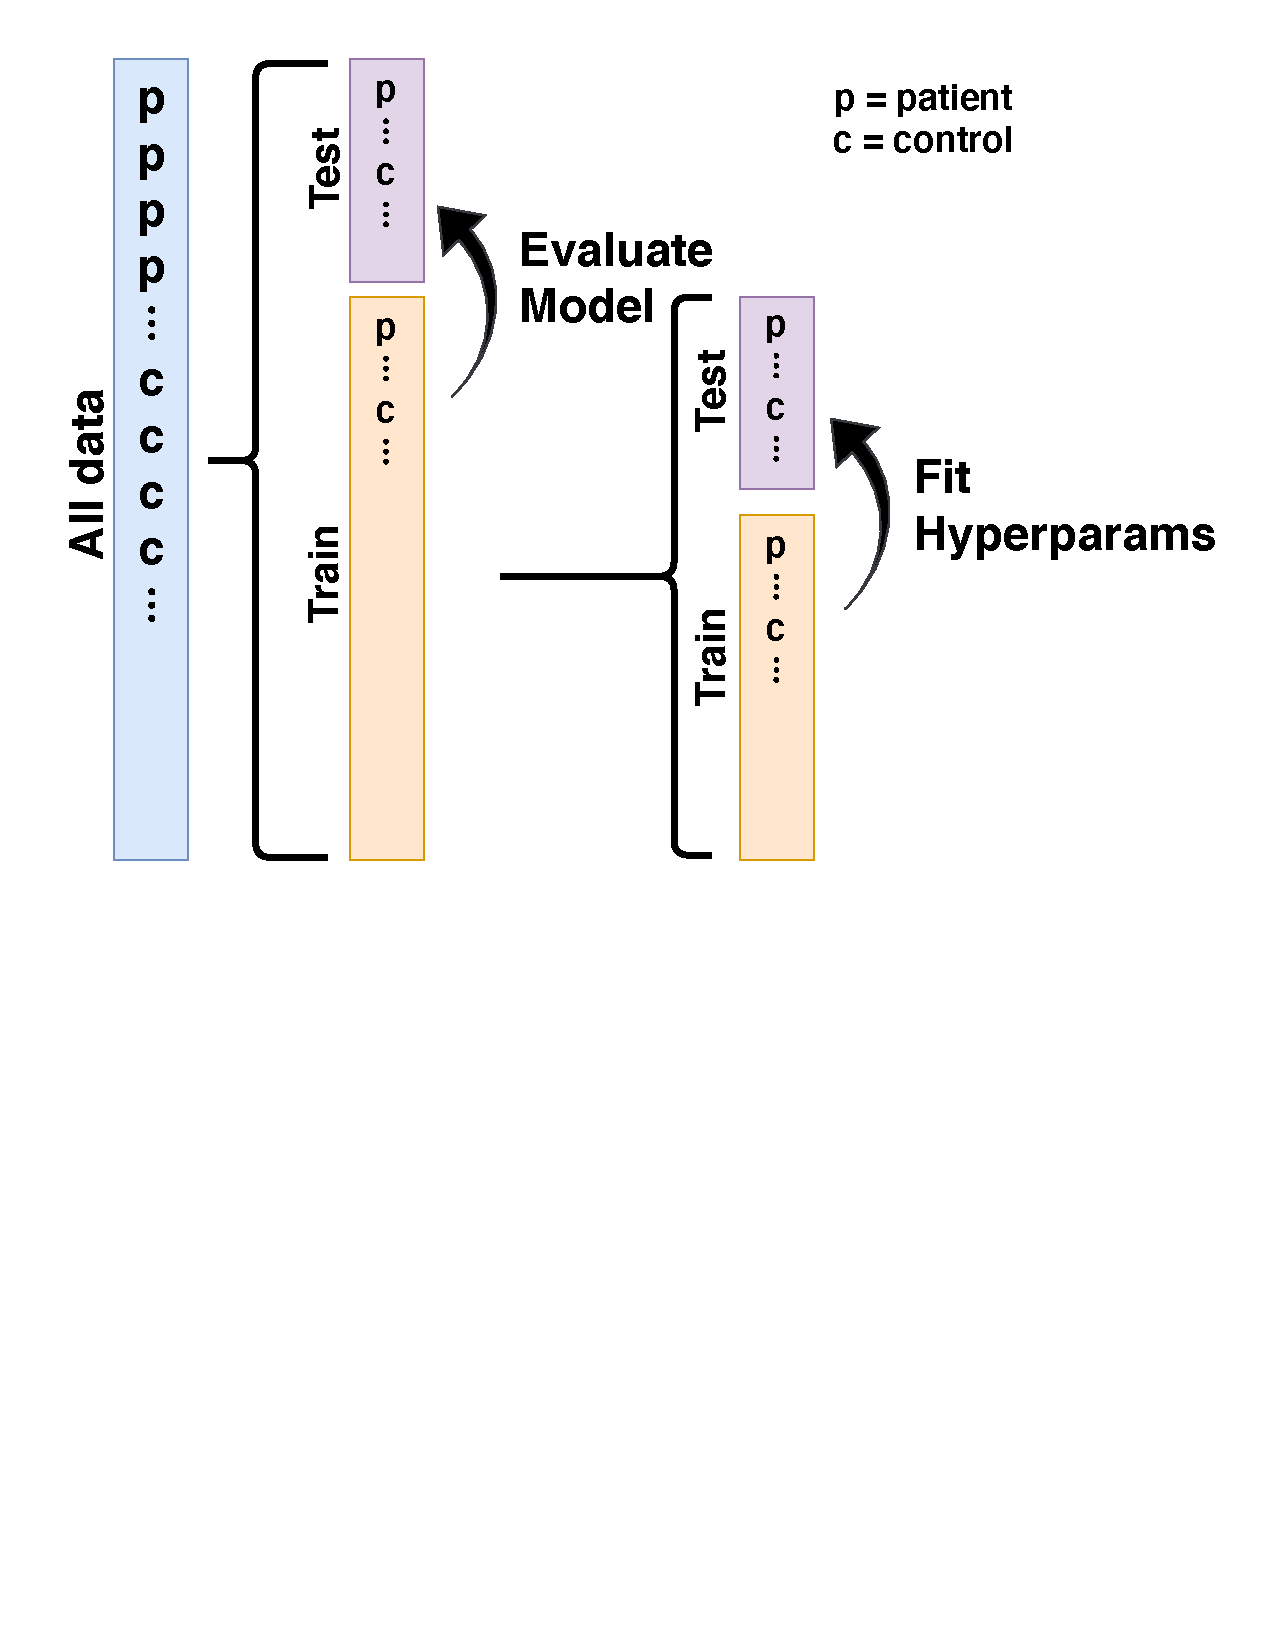
\includegraphics[width=\columnwidth]{nested-cross-validation.pdf}
    \caption{{\bf Nested cross-validation}
        \label{fig:nested-cross-val}
        We evaluate model quality using a nested $k$-fold cross validation
        scheme. At level-0, the input data is decomposed into $k_0$ shuffled
        groups and optimal hyperparameters are found for the level-0 training
        set. To avoid overfitting, the optimal hyperparameters are themselves
        evaluated using a cross-validation scheme taking place at level-1 of
        the decomposition, where each level-0 training set is further
        decomposed into $k_1 = 3$ shuffled groups. In the classification
        case, the training and test splits are stratified by diagnosis. For
        the ALS and WH data, $k_0 = 10$, while for the HBN and Cam-CAN data,
        $k_0 = 5$.
    }
\end{figure}

Because the SGL is not specific to tractometry, we implemented its solution as
a general-purpose Python package called \texttt{groupyr} \cite{groupyr}.
\texttt{Groupyr} solves the cost function in \cref{eq:sgl} using proximal
gradient descent \cite{parikh2014proximal} by implementing a custom proximal
operator and relying on the C-OPT optimization library \cite{copt}, providing
a fitted SGL model as a scikit-learn compatible estimator \cite{sklearn_api}.
\texttt{Groupyr} also selects the hyperparameters $\alpha$ and $\lambda$ that
yield the best cross-validated performance using either
\begin{enumerate*}[%
    label=(\roman*),%
    before=\unskip{: },%
    itemjoin={{, }},%
    itemjoin*={{, or }}]
    \item an exhaustive grid search of hyperparameter combinations
    \item sequential model based optimization using the scikit-optimize
    library \cite{scikit_optimize}.
\end{enumerate*}

To objectively evaluate model performance and guard against over-fitting,
we used a nested cross-validation scheme, which is depicted for the binary
classification case in \cref{fig:nested-cross-val}. The subjects (i.e. rows
of the feature matrix $\mathbf{X}$ in \cref{main:fig:methods:group-structure}
and \cref{eq:lm}) are first shuffled and then decomposed into $k_0$ batches,
hereafter referred to as folds. For the ALS and WH datasets, we used $k_0 =
10$ and for the HBN and Cam-CAN datasets, $k_0 = 5$. For each unique fold, we
hold that fold out as the test\textsubscript{0} set and let the remaining
data comprise the train\textsubscript{0} set, with the subscript indicating
the depth of the nested decomposition. We further decompose each
train\textsubscript{0} set into three folds, and again for each unique fold,
we hold out that fold as the test\textsubscript{1} set and let the remaining
data comprise the train\textsubscript{1} set. At level-1 of the
decomposition, we fit an SGL model using fixed regularization meta-parameters
$\alpha$ and $\lambda$, training the model using train\textsubscript{1} and
evaluating the fit on test\textsubscript{1}. We find the optimal values for
$\alpha$ and $\lambda$ using sequential model-based optimization, implemented
using the scikit-optimize \verb|BayesSearchCV| class\cite{scikit-optimize}.
For continuous numerical $y$, \verb|BayesSearchCV| searches for
meta-parameter values that maximize the $R^2$ averaged over test sets. For
binary categorical $y$ \verb|BayesSearchCV| seeks to maximize the
classification accuracy. Using hyperoptimization, we find optimal
regularization parameters and $\hat{\beta}$ for each train\textsubscript{0}
set and then use those to predict values for data in test\textsubscript{0}.
Thus each subject in the dataset has a predicted phenotype derived from a
model that never saw its particular subject's data. In the classification
case, the shuffling into folds is stratified such that each fold has a
population that preserves the percentage of each class found in the larger
input data.

For each dataset, we also perform a randomization test by training similar
models on copies of the data for which the rows of the target variable $y$
have been shuffled while the feature matrix $\mathbf{X}$ remains the same.
This effectively destroys any relationship between the diffusion data and the
outcome. Indeed, all of our models perform no better than random guessing.
One should expect this since any better performance might indicate data
leakage between train and test sets \cite{kaufman2012leakage} or other common
machine learning pitfalls.

\subsection{Software implementation}

The full software implementation of the SGL approach presented here is available
in a Python software package called \texttt{AFQ-Insight}, which is developed
publicly in \url{https://github.com/richford/afq-insight}.
The version of the code used to produce the results herein is also available in
\url{https://doi.org/10.5281/zenodo.3585942}\todo{Update version here}.
AFQ-Insight reads the target and feature data that has been processed by AFQ
from comma separated value (CSV) files conforming to the AFQ-Browser data
format \cite{yeatman2018browser} and represents them internally as
\lstinline{DataFrame} objects from the pandas Python library
\cite{mckinney2010data}. The software provides different options for imputing
missing data in the feature matrix. Missing interior nodes are imputed using
linear interpolation. For missing exterior nodes, the user may choose between
linear extrapolation and constant forward- or back-fill. Imputation uses only
values from adjacent nodes in the same white matter bundle in the same
subject so there is no danger of data leakage from other subjects. It uses
the scikit-learn \cite{scikit-learn} library to decompose input data into
separate test and train datasets, to scale each feature to have zero mean and
unit variance, and to evaluate each fit in the hyperparameter search using
appropriate classification and regression metrics such as accuracy, area
under the receiver operating curve (AUC ROC), and coefficient of
determination ($R^2$). Internally, \texttt{AFQ-Insight} uses the \texttt{groupyr} software library \cite{groupyr} mentioned above to solve the SGL.


\section{Bundle and coefficient profiles}
\label{sec:bundle-profiles}

Here, we present the bundle profiles and $\hat{\beta}$ coefficients
for each dataset. Throughout this section, diffusion metrics are plotted
along the length of eighteen bundles:
right corticospinal (CSTR),
left corticospinal (CSTL),
right uncinate (UNCR),
left uncinate (UNCL),
left inferior fronto-occipital fasciculus (IFOL),
right inferior fronto-occipital fasciculus (IFOR),
right arcuate (ARCR),
left arcuate (ARCL),
right thalamic radiation (ATRR),
left thalamic radiation (ATRL),
right cingulum cingulate (CGCR),
left cingulum cingulate (CGCL),
callosum forceps major (CFP),
callosum forceps minor (CFA),
right inferior longitudinal fasciculus (ILFR),
left inferior longitudinal fasciculus (ILFL),
right superior longitudinal fasciculus (SLFR),
and left superior longitudinal fasciculus (SLFL).
We display results for two different diffusion metrics: fractional anisotropy
(FA) and mean diffusivity (MD), which are extracted from different diffusion
models depending on the dataset: diffusion tensor imaging (DTI) for the ALS
and WH datasets and diffusion kurtosis imaging (DKI) for the HBN and Cam-CAN
datasets \cite{jensen2005diffusion}. The diffusion metric is always plotted
on the left $y$-axis while the $\hat{\beta}$ coefficients are displayed on
the twin axis on the right-hand-side. The scale of the $\hat{\beta}$-axis is
shared between the FA and MD metrics so that one can compare the relative
imporance of each metric.

\subsection{ALS bundle profiles}

\begin{figure*}
    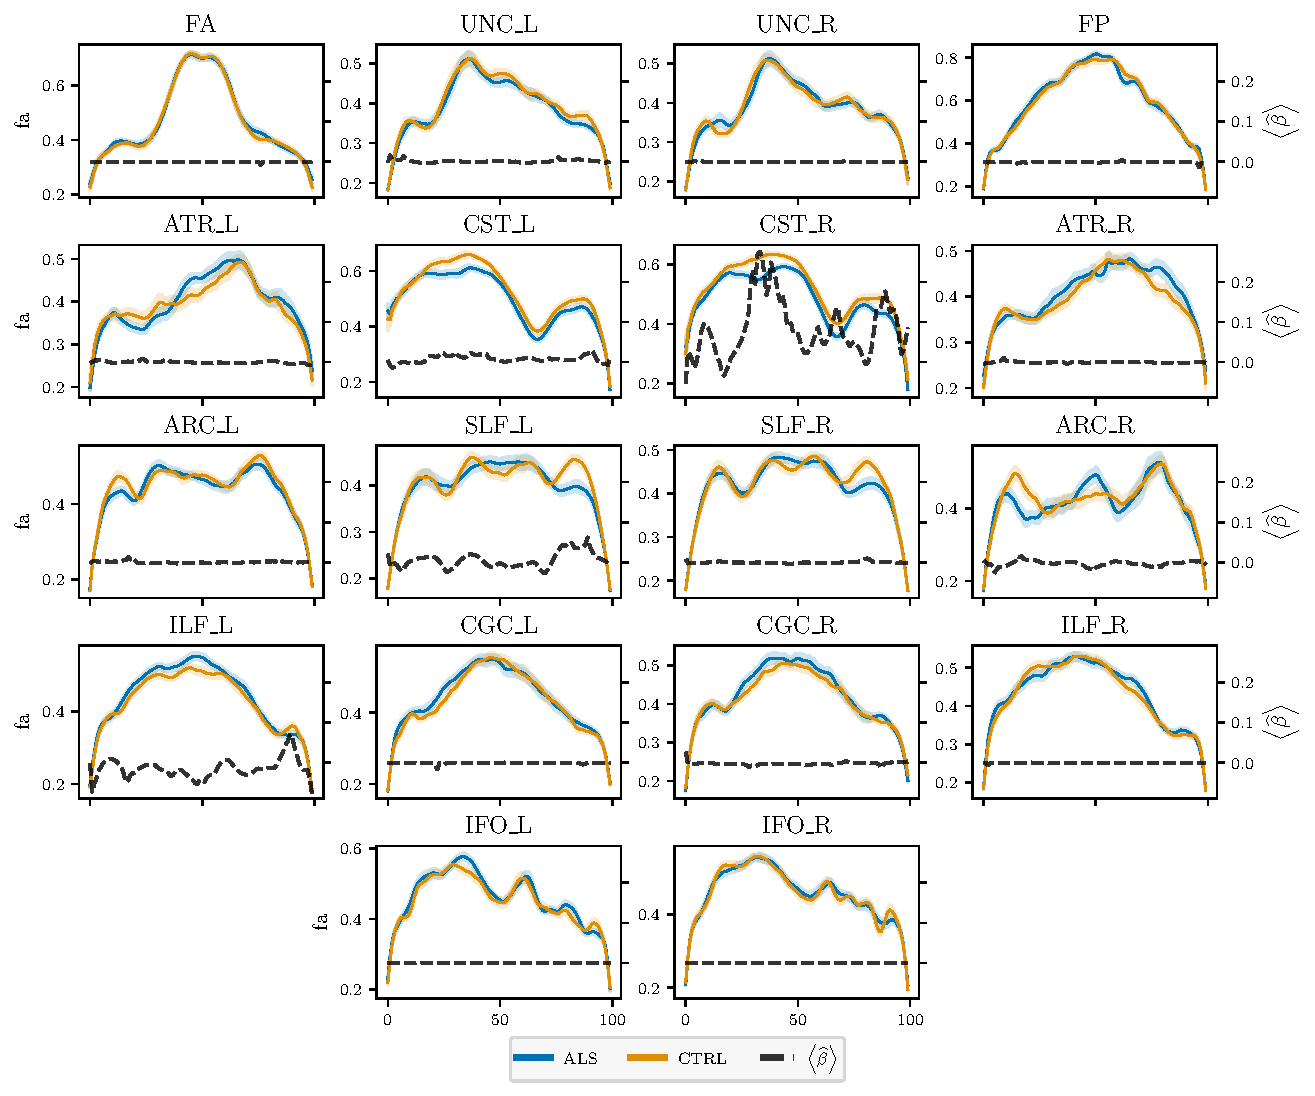
\includegraphics[width=\textwidth]{sarica_coefs_profiles_fa.pdf}
    \caption{%
        {%
            \bf Fractional anisotropy (FA) bundle profiles and $\hat{\beta}$
            coefficients for ALS classification.
        }
        \label{fig:als-bp:fa}
    }
\end{figure*}

\Cref{fig:als-bp:fa,fig:als-bp:md} show the bundle profiles and regression
coefficients for the ALS dataset FA and MD metrics, respectively. These
figures reinforce the findings in the main text that ALS is localized to the
corticospinal tract. In this study, SGL selected the right corticospinal
tract (CSTR) as important and regularized coefficients in the CSTL. Yet,
\cref{fig:als-bp:fa} also shows group FA differences in the CSTL. This
highlighted a potential drawback of the SGL method, discussed in the main
text in the context of age regression. Namely, SGL is not guaranteed to
identify \emph{all} important features. In this case, if the diagnostic
signal in the CSTL is redundant to that in the CSTR, SGL will regularize the
CSTL features, thereby reducing its sparsity penalty without any
corresponding increase in loss. This parsimony cuts both ways; it is a
feature of the method when one seeks an efficient predictive model, but is a
disadvantage of the method when one wants an exhaustive explanation of feature
importance. We will use the phrase ``parsimony pitfall'' to refer to the
case when SGL regularizes away redundant but obviously important features.

\begin{figure*}
    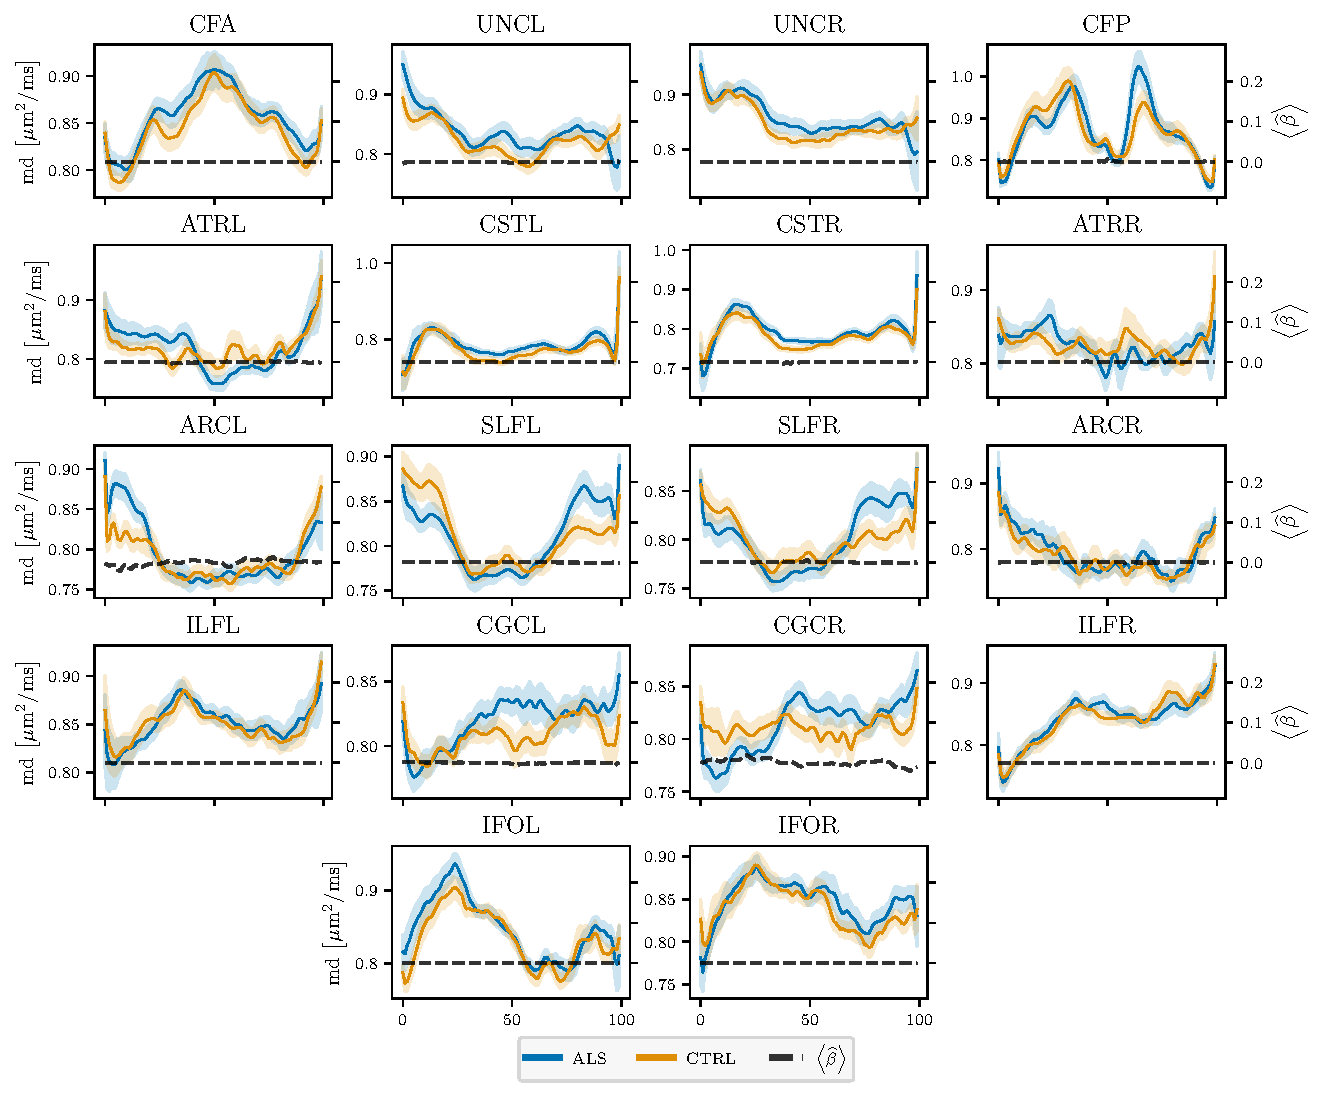
\includegraphics[width=\textwidth]{sarica_coefs_profiles_md.pdf}
    \caption{%
        {%
            \bf Mean diffusivity (MD) Bundle profiles and $\hat{\beta}$
            coefficients for ALS classification.
        }
        \label{fig:als-bp:md}
    }
\end{figure*}

\subsection{WH bundle profiles}

\begin{figure*}
    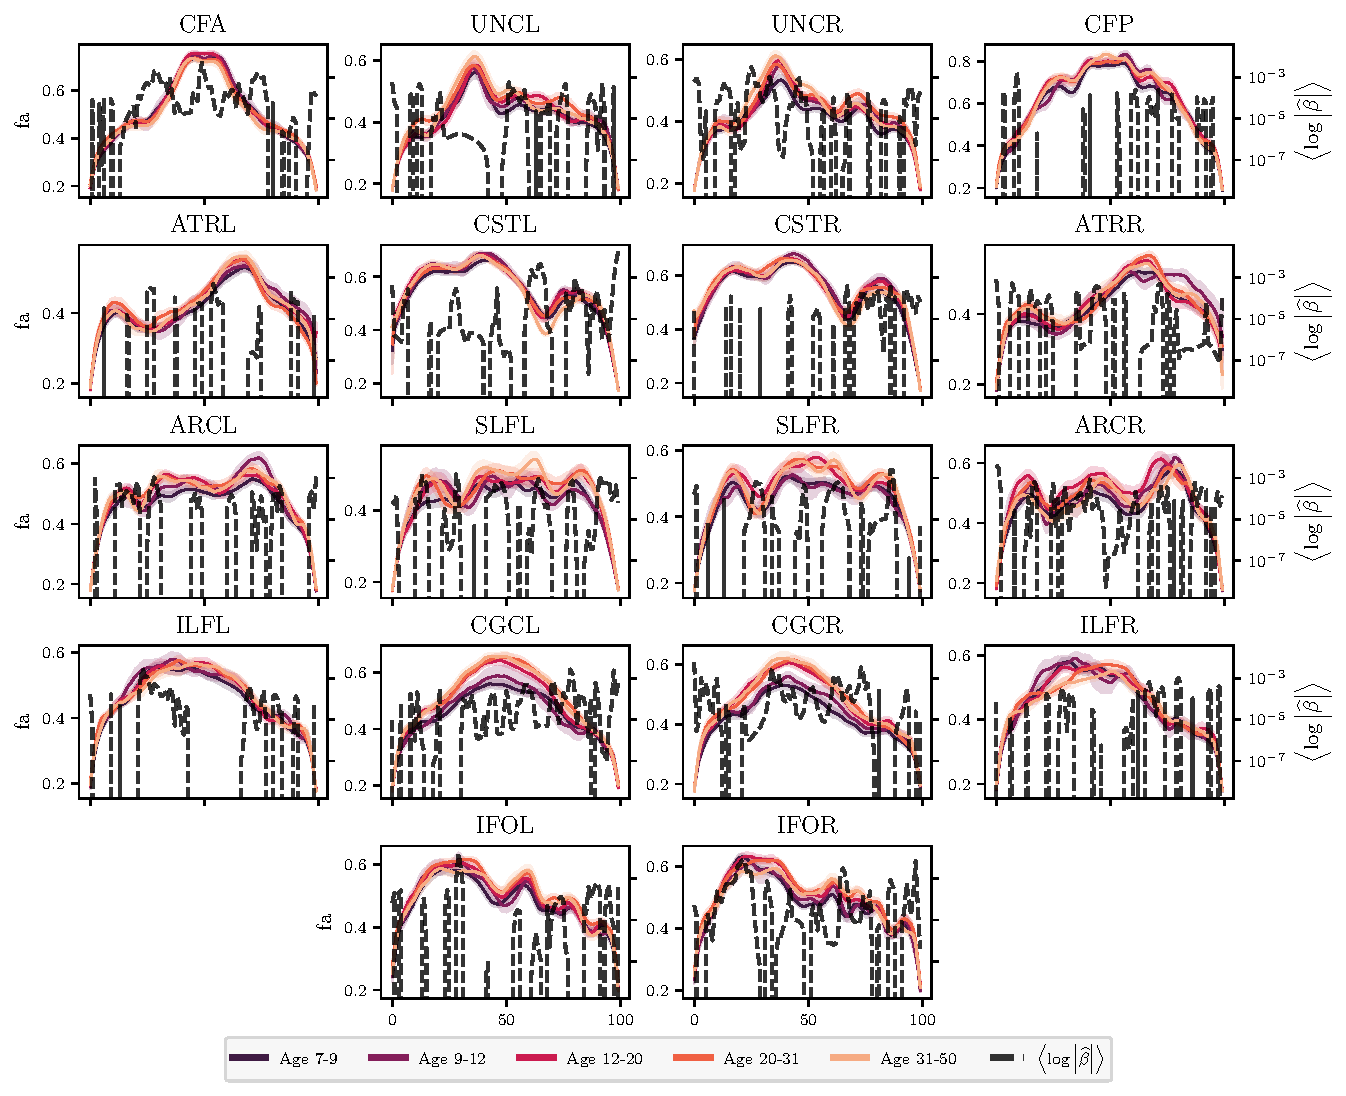
\includegraphics[width=\textwidth]{wh_coefs_profiles_fa.pdf}
    \caption{%
        {%
            \bf Fractional anisotropy (FA) bundle profiles and $\hat{\beta}$
            coefficients for age regression in the WH dataset.
        }
        \label{fig:wh-bp:fa}
    }
\end{figure*}

\Cref{fig:wh-bp:fa,fig:wh-bp:md} show the bundle profiles and regression
coefficients for the WH dataset. In contrast to the ALS classification case,
the $\hat{\beta}$ coefficients are distributed widely through the brain, supporting
the interpretation that aging is a large and continuous whole-brain process.
These figures also show that SGL behaves much more like the lasso than the group
lasso, as discussed in the main text. The parsimony pitfall is most evident in
the IFOL and IFOR bundles in \cref{fig:wh-bp:md}.

\begin{figure*}
    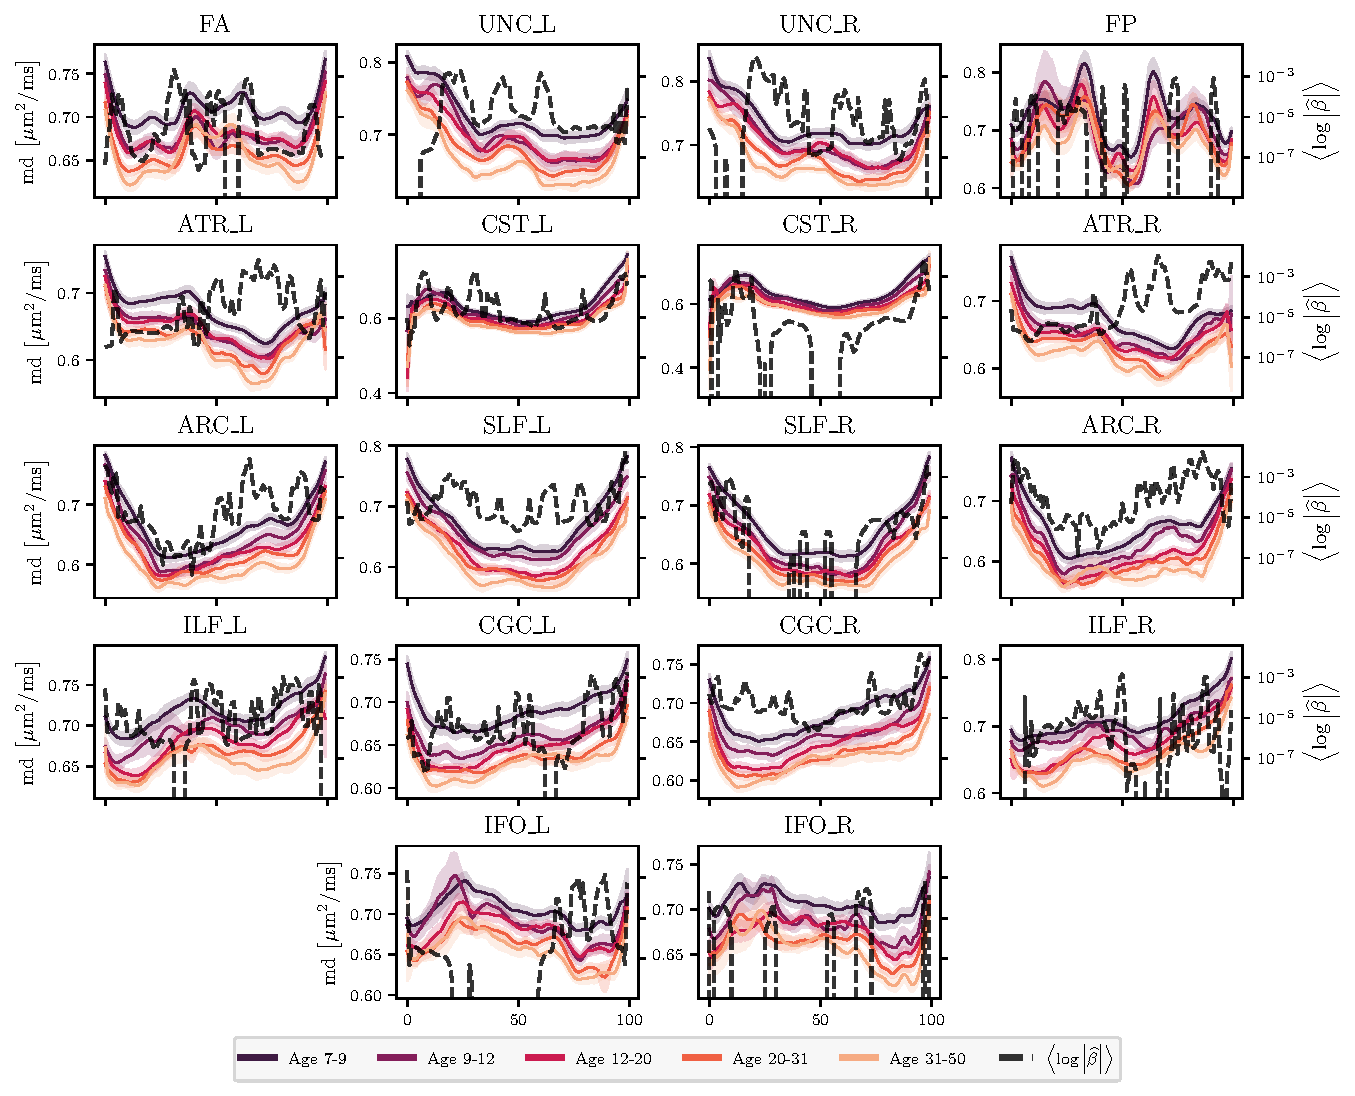
\includegraphics[width=\textwidth]{wh_coefs_profiles_md.pdf}
    \caption{%
        {%
            \bf Mean diffusivity (MD) bundle profiles and $\hat{\beta}$
            coefficients for age regression in the WH dataset.
        }
        \label{fig:wh-bp:md}
    }
\end{figure*}

\subsection{HBN bundle profiles}

\begin{figure*}
    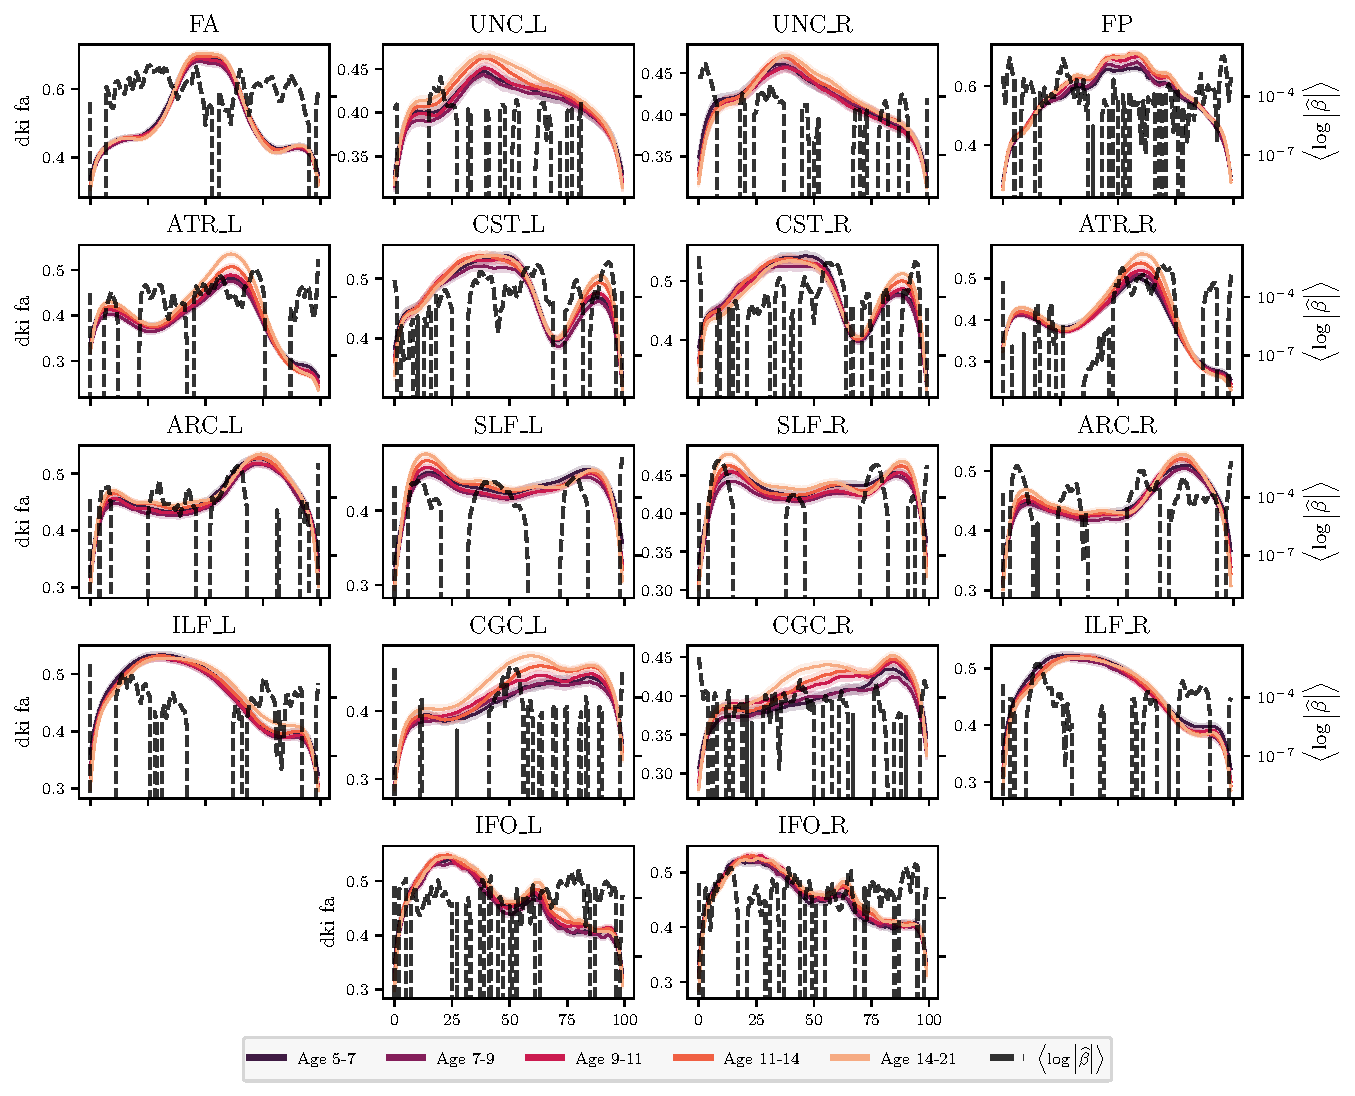
\includegraphics[width=\textwidth]{hbn_coefs_profiles_fa.pdf}
    \caption{%
        {%
            \bf Fractional anisotropy (FA) bundle profiles and $\hat{\beta}$
            coefficients for age regression in the HBN dataset.
        }
        \label{fig:hbn-bp:fa}
    }
\end{figure*}

\Cref{fig:hbn-bp:fa,fig:hbn-bp:md} show the bundle profiles and regression
coefficients for the HBN dataset. Like the WH dataset, the $\hat{\beta}$
coefficients are distributed widely through the brain and SGL behaves more
like the lasso than the group lasso. In contrast the the WH results,
the bundle profiles show different behaviors. For example the SLFL and SLFR
bundle profiles in \cref{fig:wh-bp:md} and \cref{fig:hbn-bp:md} have
different concavity. This is unsurprising, however, given the differences
between these datasets
\begin{enumerate*}[%
    label=(\roman*),%
    before=\unskip{: },%
    itemjoin={{, }},%
    itemjoin*={{, and }}]
    \item different diffusion models, with DTI for the WH dataset and DKI for
    the HBN dataset
    \item different age ranges and distributions (which is evident in the
    figure legends), with HBN being a developmental dataset, while WH is a
    lifespan maturation dataset
    \item different anatomical extents, with the WH streamlines truncated to
    remain with the bundle's bounding regions of interest (the default
    behavior in the legacy \texttt{mAFQ}) and the HBN streamlines allowed
    to retain their full extent from whole-brain tractography (the default
    behavior in \texttt{pyAFQ}).
\end{enumerate*}
Thus, one should use caution when comparing bundle profiles and $\hat{\beta}$
coefficients between the WH, HBN, and Cam-CAN models.
The parsimony pitfall is most evident in the UNCL, UNCR, ARCL, SLFL, and
SLFR bundles in \cref{fig:hbn-bp:md}.

\begin{figure*}
    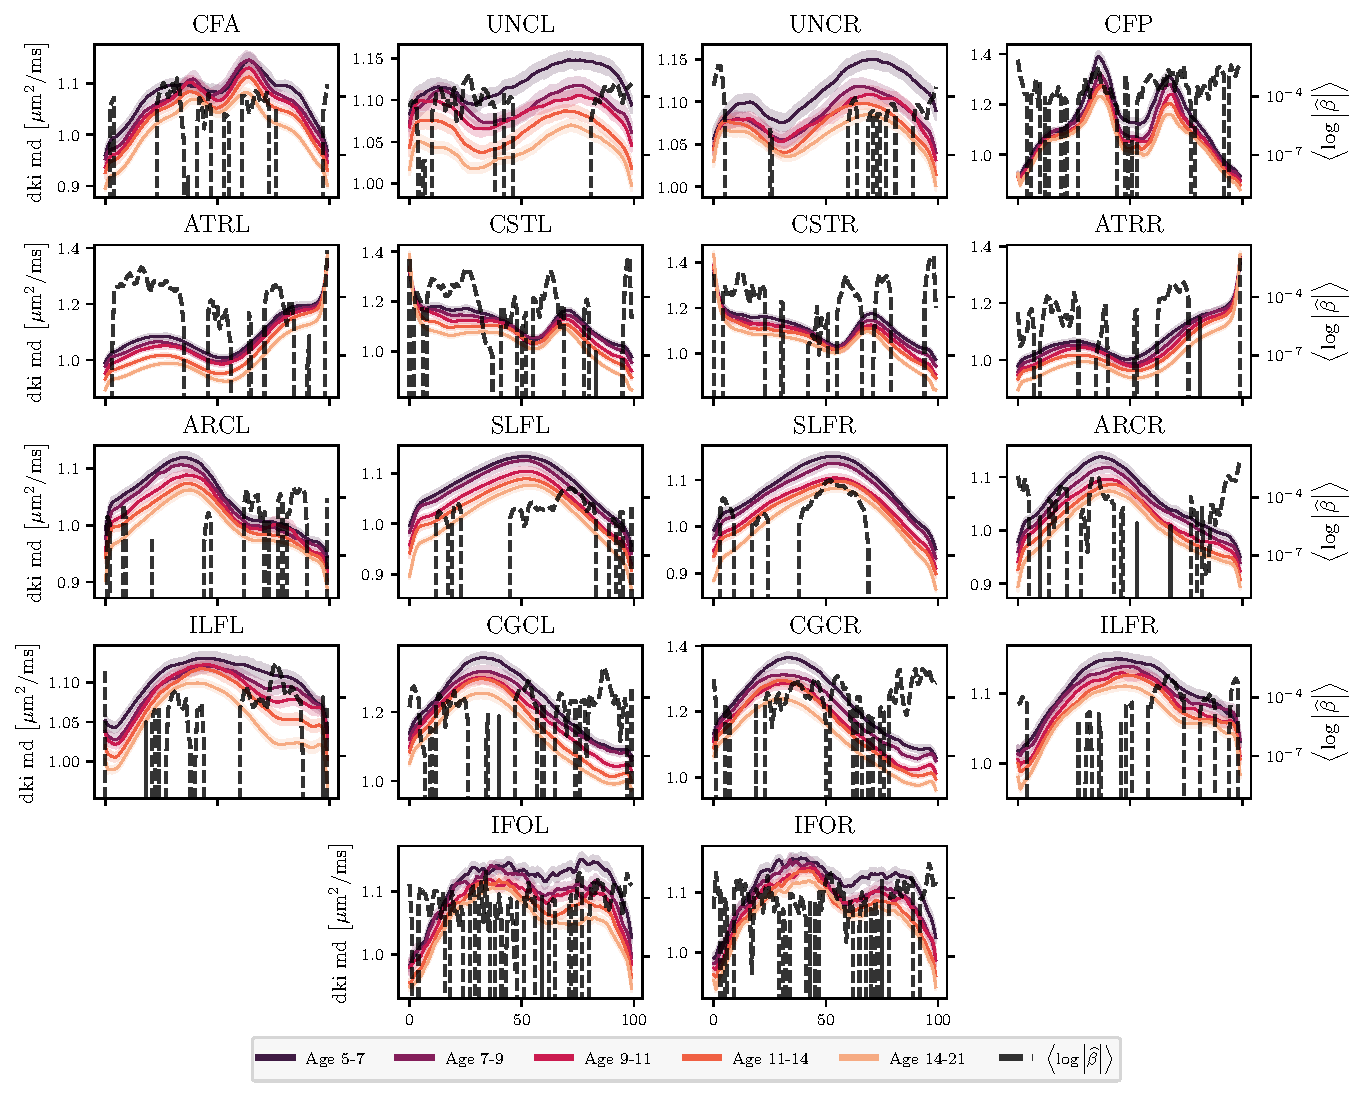
\includegraphics[width=\textwidth]{hbn_coefs_profiles_md.pdf}
    \caption{%
        {%
            \bf Mean diffusivity (MD) bundle profiles and $\hat{\beta}$
            coefficients for age regression in the HBN dataset.
        }
        \label{fig:hbn-bp:md}
    }
\end{figure*}

\subsection{Cam-CAN bundle profiles}

\begin{figure*}
    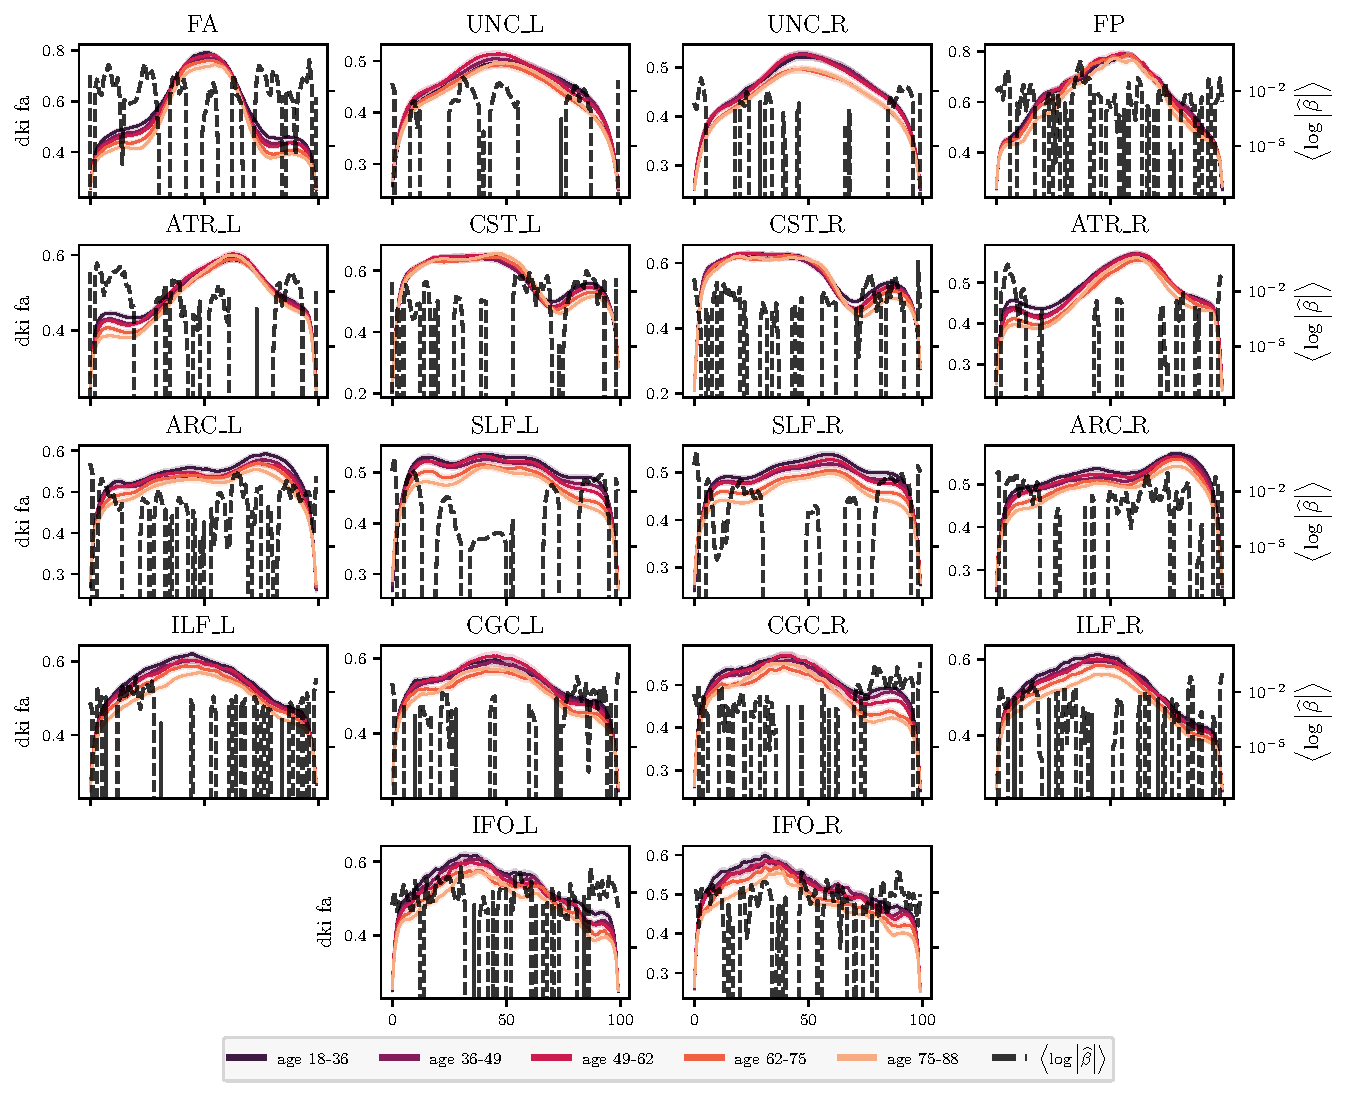
\includegraphics[width=\textwidth]{cc_coefs_profiles_fa.pdf}
    \caption{%
        {%
            \bf Fractional anisotropy (FA) bundle profiles and $\hat{\beta}$
            coefficients for age regression in the Cam-CAN dataset.
        }
        \label{fig:cc-bp:fa}
    }
\end{figure*}

\Cref{fig:cc-bp:fa,fig:cc-bp:md} show the bundle profiles and regression
coefficients for the Cam-CAN dataset. Like the WH and HBN datasets, the
$\hat{\beta}$ coefficients are distributed widely through the brain and SGL
behaves more like the lasso than the group lasso. As before, one must be
cautious about comparing bundle profiles and $\hat{\beta}$ coefficients
between models. While the HBN and Cam-CAN datasets share the same diffusion
model and refrain from clipping streamlines, the age distributions for the
two are roughly disjoint, with the WH age distribution straddling the two.
The parsimony pitfall is again evident in the UNCL, UNCR, ARCL, SLFL, and
SLFR bundles in \cref{fig:cc-bp:md}.

\begin{figure*}
    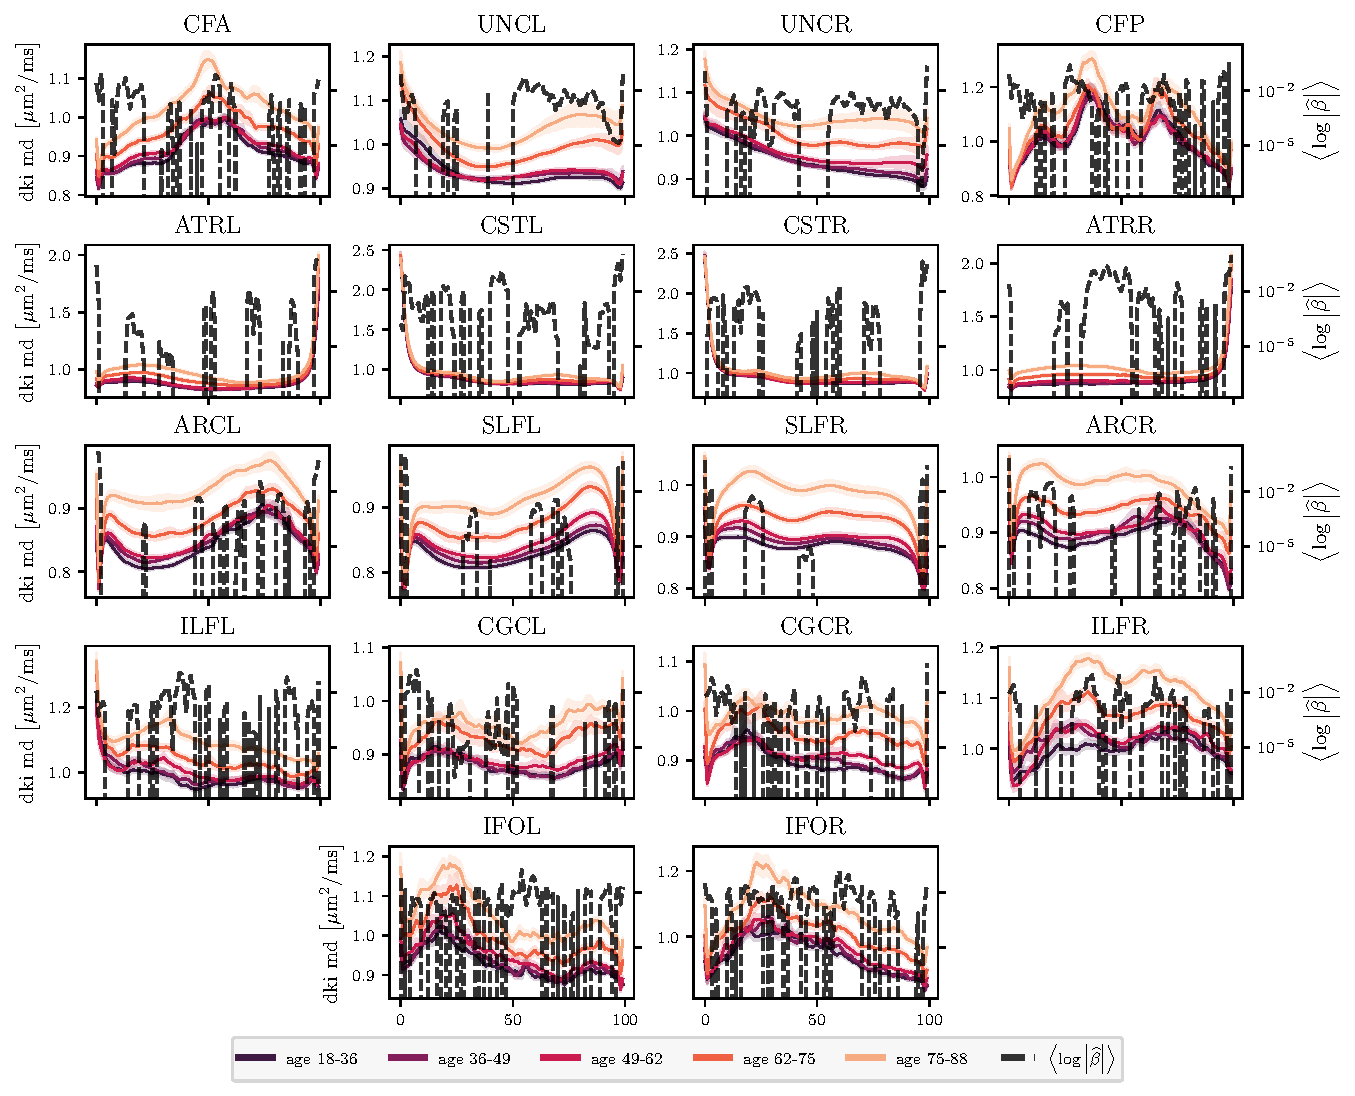
\includegraphics[width=\textwidth]{cc_coefs_profiles_md.pdf}
    \caption{%
        {%
            \bf Mean diffusivity (MD) bundle profiles and $\hat{\beta}$
            coefficients for age regression in the Cam-CAN dataset.
        }
        \label{fig:cc-bp:md}
    }
\end{figure*}

\printfigures

\bibliographystyle{naturemag}
\bibliography{paper}

\end{document}
